\chapter{波動関数、密度行列、局所性}

\lectureoverview{ベルルの定理を後回しにするのには、本質的な理由が一つある。ベルルが何を禁じるかを問う前に、もつれとは正確に何であるかを述べなければならない。二部分系の状態は、アリスに対する一つの状態とボブに対する一つの状態に因数分解できないとき、もつれている。波動関数はその判定基準を具体的なものにし、相関はその帰結を明らかにし、一重項は決定的な例を与える。次に、縮約密度行列が、もつれた全体の一部分の完全な局所的記述となる。その道具立てを手にすると、測定はもつれを生じる相互作用として現れ、系--観測者という境界は予測を変えることなく移動でき、もつれと局所性の間の見かけの緊張は鋭く述べられる。すなわち、遠方での選択は条件付き相関を変えるが、シグナル伝達に利用できる無条件の統計量は変えない。}

\section{もつれとは実際に何を意味するか}

ベルルの定理へ直接進みたくなる。この定理は美しいが、その意義はそれが検証する構造から切り離せない。したがって、より緊急の問いは、まだ量子力学がベルル不等式に違反するかどうかではなく、もつれた状態が複合系について何を述べているかである。

よくある言い回しは、二つのもつれた系が\emph{状態を共有する}というものである。その言い回しは何も区別していない。すべての複合系は、もつれていようといまいと、状態をもつ。区別は因数分解にある。\(A\)と\(B\)がヒルベルト空間\(\mathcal H_A\)と\(\mathcal H_B\)をもつなら、その対の状態は
\begin{equation}
\mathcal H_{AB}=\mathcal H_A\otimes\mathcal H_B.
\end{equation}
に属する。純粋状態は
\begin{equation}
\ket{\Psi}_{AB}=\ket{\psi}_A\otimes\ket{\phi}_B.
\label{eq:l7-product-state}
\end{equation}
と書けるとき積状態である。そのような因数の対が存在しないなら、\(\ket{\Psi}_{AB}\)はもつれている。

\begin{classroomqa}
\audiencequestion{もつれとは、単に両方の系が一つの状態ベクトルの中に現れることを意味するのですか。}
\lecturerresponse{いいえ。積状態もまた、対全体のヒルベルト空間に属する。もつれとは、全体のベクトルがアリスに対する一つのベクトルとボブに対する一つのベクトルの積として書けないという、より強い、基底に依存しない主張である。}
\end{classroomqa}

\begin{classroomqa}
\audiencequestion{巧みな基底の変更によって、もつれた状態を積状態に変えることはできますか。}
\lecturerresponse{その基底の変更が局所的、つまりアリスに対する一つの基底変更とボブに対するもう一つの基底変更であるなら、できない。局所的な基底変更は各因数の座標を変えるが、状態が因数分解するかどうかは変えない。結合ヒルベルト空間の完全に任意の基底はテンソル積構造を隠しうるが、どの物理的自由度がアリスとボブに属するかは変えない。}
\end{classroomqa}

\section{ヒルベルト空間における座標としての波動関数}

\emph{波動関数}という語には、その数学的定義の一部ではない歴史的なイメージが伴う。波動関数とは、選ばれた基底における状態ベクトルの座標表示である。可換な観測量の完全集合が同時固有ベクトル
\begin{equation}
\ket{a,b,c,\ldots}.
\end{equation}
をもつとする。ラベルは完全でなければならない。すなわち、それらを合わせると基底のすべてのベクトルを区別する。すると
\begin{align}
\ket{\Psi}
&=\sum_{a,b,c,\ldots}
\ket{a,b,c,\ldots}
\braket{a,b,c,\ldots}{\Psi} \\
&=\sum_{a,b,c,\ldots}
\psi(a,b,c,\ldots)\ket{a,b,c,\ldots},
\label{eq:l7-wavefunction-expansion}
\end{align}
ここで
\begin{equation}
\psi(a,b,c,\ldots)
=\braket{a,b,c,\ldots}{\Psi}.
\label{eq:l7-wavefunction-definition}
\end{equation}
である。連続的なラベルに対しては、対応する和は積分になる。

\begin{figure}[htbp]
\centering
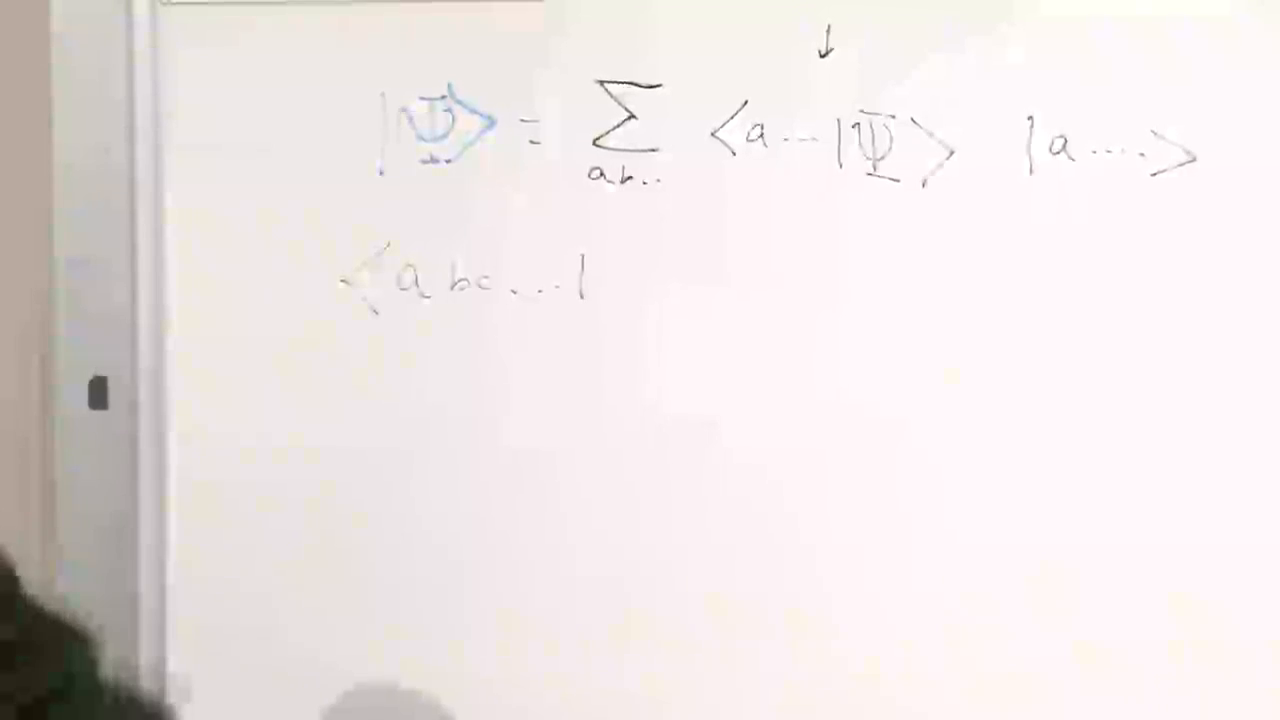
\includegraphics[width=0.88\textwidth]{lecture_07_figure_01.png}
\caption{完全な基底における状態の係数の集合としての波動関数。}
\lectureframe{00:07:00}
\end{figure}

三次元空間中の粒子に対しては、可換なラベルは\(x,y,z\)であり、
\begin{equation}
\psi(x,y,z)=\braket{x,y,z}{\Psi}
\end{equation}
はSchr\"odingerのよく知られた位置空間の波動関数である。\(\sigma_z\)基底における一つのスピンに対しては、波動関数は単に対
\begin{equation}
\psi(u)=\braket{u}{\Psi},
\qquad
\psi(d)=\braket{d}{\Psi}.
\end{equation}
である。二つのスピンに対しては、二つのラベルが必要である。
\begin{equation}
\Psi(a,b)=\braket{a,b}{\Psi},
\qquad
a,b\in\{u,d\}.
\label{eq:l7-two-spin-wavefunction}
\end{equation}
この定義のどこにも、空間における文字通りの波は必要ない。

\begin{classroomqa}
\audiencequestion{波動関数の基底を変えることはフーリエ変換ですか。}
\lecturerresponse{フーリエ変換は、位置表示と運動量表示の間の特定の基底変更である。より一般には、正規直交基底のあらゆる変更は座標のユニタリ変換である。\(\sigma_z\)基底から\(\sigma_x\)基底への移行はフーリエ変換に類似しているが、それは位置--運動量の積分変換ではなく、有限次元のユニタリ行列である。}
\end{classroomqa}

\begin{classroomqa}
\audiencequestion{基底変更の下で波動関数が変われば、物理的状態は変わったのですか。}
\lecturerresponse{いいえ。ケット\(\ket{\Psi}\)が抽象的な状態である。数\(\psi(a,b,c,\ldots)\)は、選ばれた基底におけるその座標である。座標を変えることはそれらの数を変えるが、ベクトルとすべての物理的予測は変えない。}
\end{classroomqa}

\section{成分による期待値}

密度行列を導入する前に、期待値の成分構造を明らかにしておく。\(L\) を観測量とし、その行列要素を
\begin{equation}
L_{a'a}=\bra{a'}L\ket{a}.
\label{eq:l7-matrix-elements}
\end{equation}
とする。\(\ket{\Psi}=\sum_a\psi(a)\ket{a}\) ならば、
\begin{align}
\expect{L}
&=\bra{\Psi}L\ket{\Psi} \\
&=\sum_{a',a}
\psi^*(a')\bra{a'}L\ket{a}\psi(a) \\
&=\sum_{a',a}\psi^*(a')L_{a'a}\psi(a).
\label{eq:l7-expectation-components}
\end{align}

\begin{figure}[htbp]
\centering
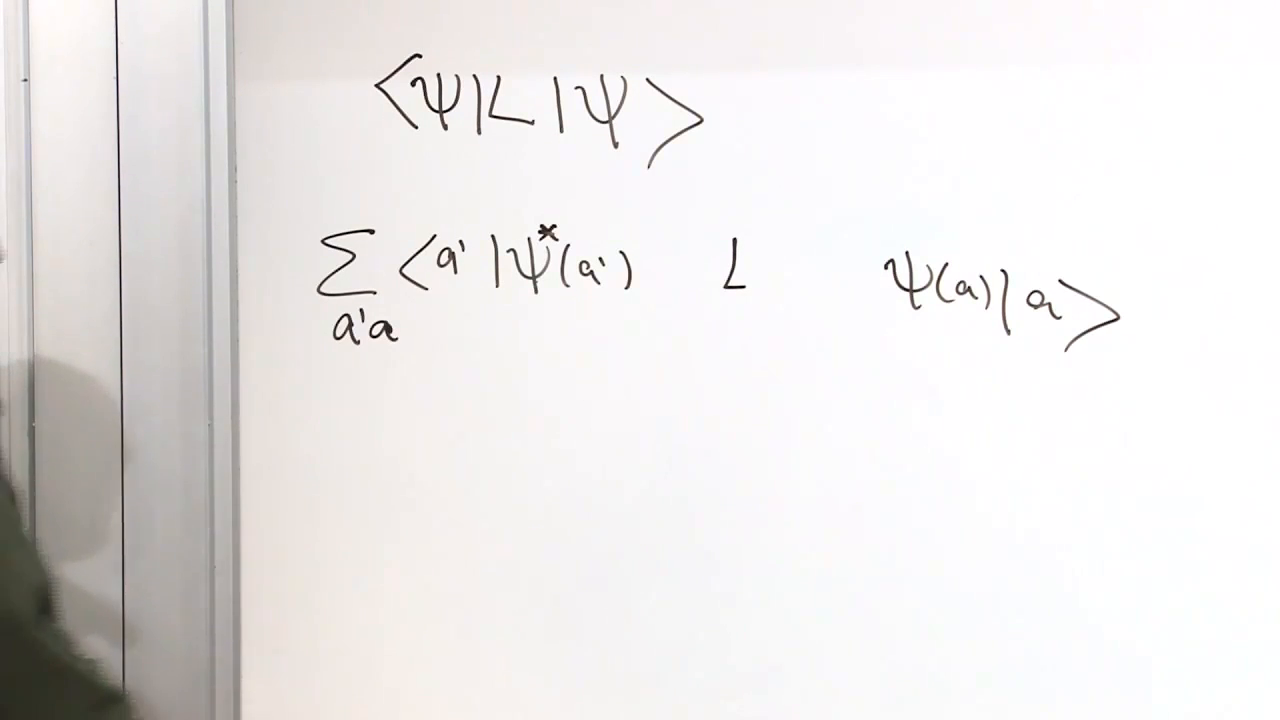
\includegraphics[width=0.88\textwidth]{lecture_07_figure_02.png}
\caption{期待値のサンドイッチを波動関数の係数と行列要素に展開したもの。}
\lectureframe{00:14:08}
\end{figure}

ここで系をアリスの部分とボブの部分に分ける。\(a\) をアリスの完全基底のラベル、\(b\) をボブの完全基底のラベルとする：
\begin{equation}
\ket{\Psi}_{AB}
=\sum_{a,b}\Psi(a,b)\ket{a,b}.
\label{eq:l7-composite-expansion}
\end{equation}
アリスにのみ属する観測量は、合成空間上で
\begin{equation}
L_A=L\otimes I_B,
\end{equation}
と表されるので、その行列要素は
\begin{equation}
\bra{a',b'}L_A\ket{a,b}
=L_{a'a}\delta_{b'b}.
\label{eq:l7-alice-local-matrix}
\end{equation}
である。同様に、ボブに局所的な観測量は
\begin{equation}
M_B=I_A\otimes M,
\qquad
\bra{a',b'}M_B\ket{a,b}
=\delta_{a'a}M_{b'b}.
\label{eq:l7-bob-local-matrix}
\end{equation}
の形をとる。手をつけていない因子の恒等演算子は、アリスの操作はアリスに作用し、ボブの操作はボブに作用するという数学的表現である。

式~\eqref{eq:l7-alice-local-matrix}を期待値に代入すると
\begin{equation}
\expect{L_A}
=\sum_{a',a,b}
\Psi^*(a',b)L_{a'a}\Psi(a,b).
\label{eq:l7-local-expectation}
\end{equation}
が得られる。この式にはすでに縮約密度行列が含まれている。因数分解が何をするかを見た後で、これを再編成する。

\begin{classroomqa}
\audiencequestion{式~\eqref{eq:l7-local-expectation}でボブの添字が1つしか残らないのはなぜか。}
\lecturerresponse{ボブの空間の恒等演算子が \(\delta_{b'b}\) に寄与する。それはボブ側のブラとケットのラベルを等しく設定するので、\(b',b\) に関する二重和は \(b\) に関する一重和に縮約される。}
\end{classroomqa}

\begin{classroomqa}
\audiencequestion{アリスはボブがどの基底を使うかを知る必要があるか。}
\lecturerresponse{いかなる物理的予言もボブの基底に依存しない。完全なボブ基底に関する和は恒等演算子の分解である。異なるボブ基底は個々の成分 \(\Psi(a,b)\) を変えるが、アリスの期待値は変えない。}
\end{classroomqa}

\section{積状態と相関}

積状態では、結合波動関数が因数分解する：
\begin{equation}
\Psi(a,b)=\psi_A(a)\phi_B(b).
\label{eq:l7-wavefunction-factorization}
\end{equation}
これを式~\eqref{eq:l7-local-expectation}に代入すると：
\begin{align}
\expect{L_A}
&=\sum_{a',a,b}
\psi_A^*(a')\phi_B^*(b)
L_{a'a}
\psi_A(a)\phi_B(b) \\
&=\left[
\sum_{a',a}\psi_A^*(a')L_{a'a}\psi_A(a)
\right]
\left[
\sum_b|\phi_B(b)|^2
\right] \\
&=\bra{\psi_A}L\ket{\psi_A}.
\label{eq:l7-product-local-expectation}
\end{align}
ボブの規格化により、ボブの因子は1に等しくなる。したがってアリスは、ボブの系がそもそも導入されなかった場合とまったく同じ局所統計をもつ。

\begin{figure}[htbp]
\centering
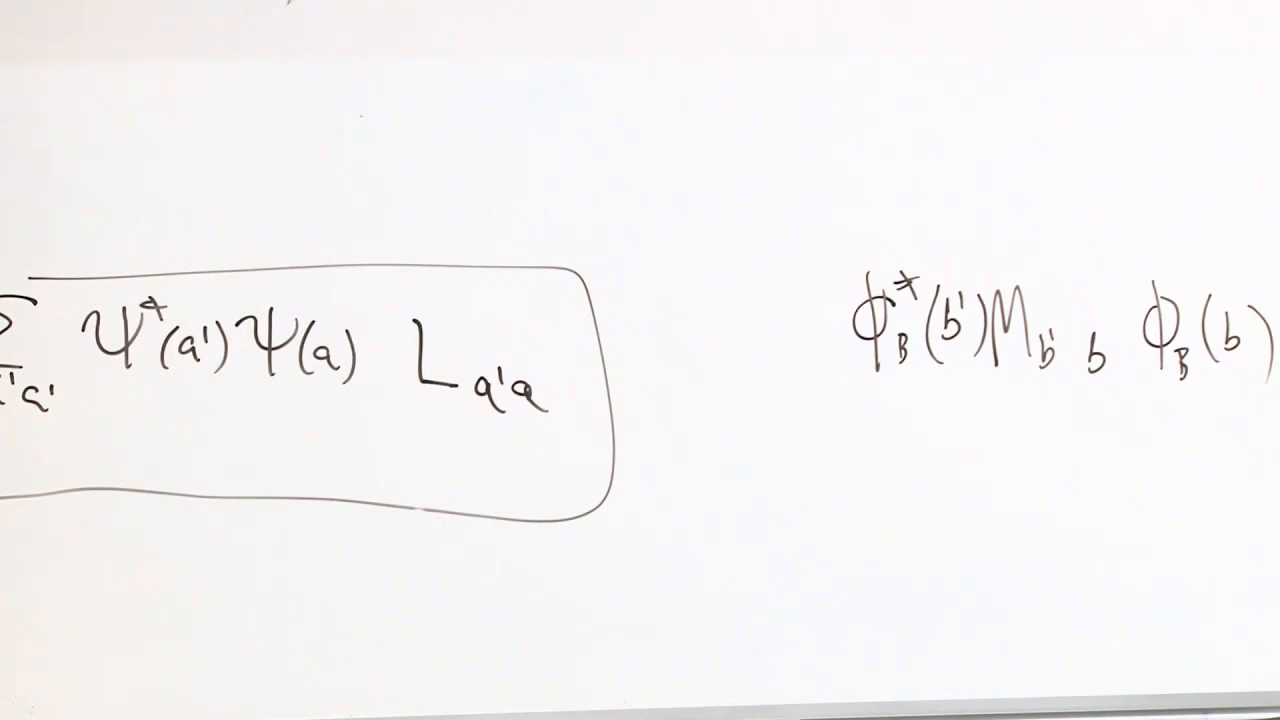
\includegraphics[width=0.88\textwidth]{lecture_07_figure_03.png}
\caption{結合波動関数の因数分解と、それに対応する局所期待値の分離。}
\lectureframe{00:29:18}
\end{figure}

アリスの観測量1つとボブの観測量1つの積は、行列要素
\begin{equation}
\bra{a',b'}L_A M_B\ket{a,b}
=L_{a'a}M_{b'b}.
\end{equation}
をもつ。積状態に対して、その期待値は分離する：
\begin{equation}
\expect{L_A M_B}
=\expect{L_A}\expect{M_B}.
\label{eq:l7-product-correlation-factorization}
\end{equation}
したがって、連結相関
\begin{equation}
C(L,M)
=\expect{L_A M_B}
-\expect{L_A}\expect{M_B}.
\label{eq:l7-connected-correlation}
\end{equation}
を定義するのが自然である。すべての積状態は、任意の局所観測量の対に対して \(C(L,M)=0\) をもつ。逆に、純粋な二部分系状態に対しては、もつれがあると、ある局所観測量の対が非零の連結相関をもつことが保証される。

\begin{classroomqa}
\audiencequestion{\(L_A M_B\) はボブが先に測定され、アリスが後に測定されることを意味するのか。}
\lecturerresponse{いいえ。演算子は状態ベクトルに作用し、装置は測定を行う。積は \(M_B\) が作用し、次に \(L_A\) が作用することを意味する。演算子は異なるテンソル因子を占めるので \([L_A,M_B]=0\) であり、したがってそれらの数学的順序は重要でない。結合期待値を推定するための実験室の手順は別の問題である。}
\end{classroomqa}

\begin{classroomqa}
\audiencequestion{選んだ相関の1つが消えていても、状態はもつれていることができるか。}
\lecturerresponse{もちろんである。1つの \(C(L,M)\) が消えることは、この特定の観測量の対が無相関であることだけを述べている。純粋状態に対して因数分解を確立するには、すべての局所相互相関が因数分解しなければならない。また、部分的な相関は、単純な一つの数の意味で部分的なもつれを意味する必要は必ずしもない。その情報は完全な縮約密度スペクトルが担っている。}
\end{classroomqa}

\begin{classroomqa}
\audiencequestion{相関のある状態はすべてもつれているのか。}
\lecturerresponse{ここで議論している純粋状態に対しては、因数分解しない相関はもつれを明らかにする。混合状態に対しては、通常の古典的相関も \(C(L,M)\neq0\) にすることができる。したがって、後の密度行列の判定基準は、全体の状態が純粋であることが知られているかどうかによって限定されなければならない。}
\end{classroomqa}

\section{一重項：部分は不定だが全体は確定}

\(\boldsymbol{\sigma}\) をボブのスピンに、\(\boldsymbol{\tau}\) をアリスのスピンに作用させる。それらの一重項状態は
\begin{equation}
\ket{S}
=\frac{1}{\sqrt2}
\left(\ket{u d}-\ket{d u}\right),
\label{eq:l7-singlet}
\end{equation}
である。ここで最初のスロットはボブのもので、2番目はアリスのものである。どちらのスピンも確定した \(z\) 成分をもたない：
\begin{equation}
\expect{\sigma_z}=0,
\qquad
\expect{\tau_z}=0.
\label{eq:l7-singlet-local-z}
\end{equation}
しかしそれらの積は確定している：
\begin{equation}
\expect{\sigma_z\tau_z}=-1.
\label{eq:l7-singlet-product-z}
\end{equation}
すべての \(z\) 測定は反対の結果を生む。

回転不変性により、この記述は方向に依存しない。任意の単位ベクトル \(\mathbf n\) に対して、
\begin{equation}
\expect{\boldsymbol{\sigma}\cdot\mathbf n}
=\expect{\boldsymbol{\tau}\cdot\mathbf n}=0,
\qquad
\expect{
(\boldsymbol{\sigma}\cdot\mathbf n)
(\boldsymbol{\tau}\cdot\mathbf n)
}=-1.
\label{eq:l7-singlet-any-axis}
\end{equation}
より一般には、
\begin{equation}
\expect{\sigma_i\tau_j}=-\delta_{ij}.
\label{eq:l7-singlet-correlation-tensor}
\end{equation}
各部分は完全に無偏極であり、一方、等しい軸の結果は完全に反相関している。

\begin{figure}[htbp]
\centering
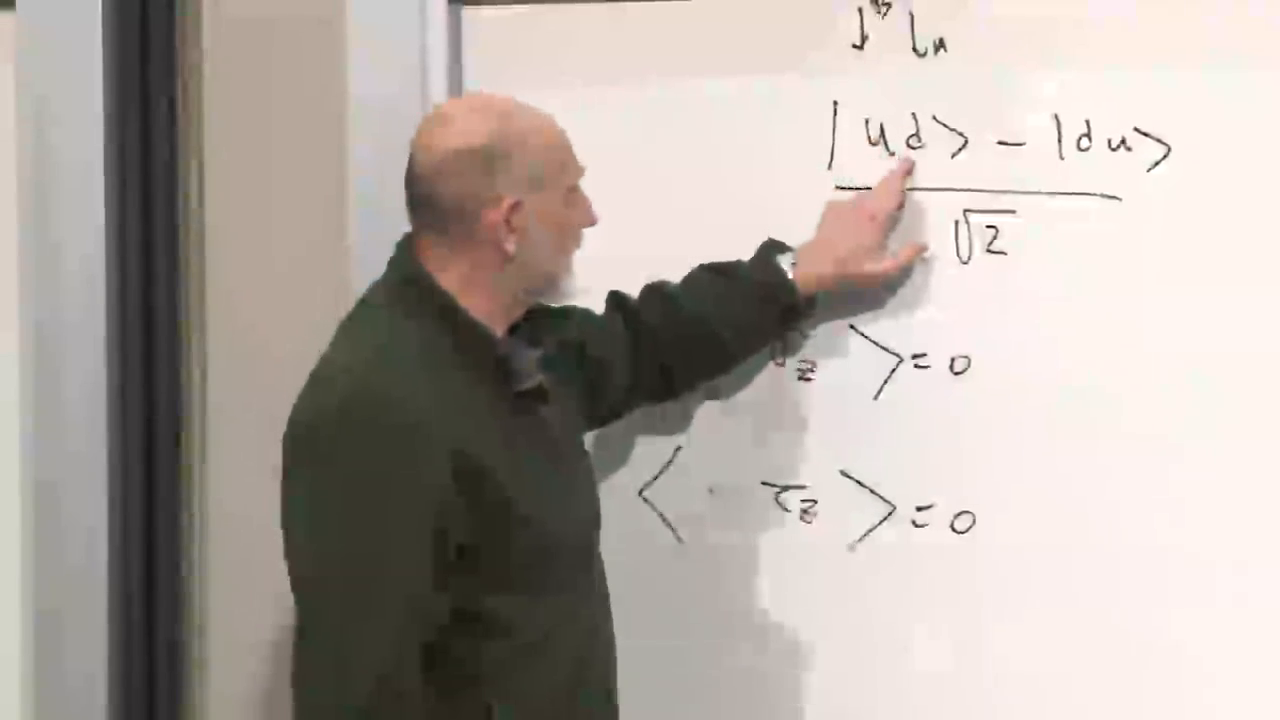
\includegraphics[width=0.88\textwidth]{lecture_07_figure_04.png}
\caption{一重項に対して、各局所スピン平均は消え、一方、等しい成分の積は \(-1\) となる。}
\lectureframe{00:38:28}
\end{figure}

これが、もつれによって生じる特徴的な反転である。孤立した純粋状態のスピンには、そのスピンが確定する方向が存在する。一重項では、どの方向によってもどちらの局所スピンも確定しない。それにもかかわらず、複合状態は純粋であり、完全に指定されている。われわれは全体について量子力学が許す限りのことを知っていながら、どちらの部分にも純粋状態を割り当てることができない。

\begin{classroomqa}
\audiencequestion{全体の状態が正確にわかっているのなら、なぜ各スピンの確定した状態を推論できないのですか。}
\lecturerresponse{一重項は積ではないからである。その係数は、ボブの振幅とアリスの振幅の積に分解されない。情報は、独立に存在する二つの局所波動関数にあるのではなく、部分間の関係にある。}
\end{classroomqa}

\begin{classroomqa}
\audiencequestion{\(\sigma_z\)のような演算子それ自体は、スピンの可能な状態なのですか。}
\lecturerresponse{いいえ。状態はベクトル、より一般には密度演算子であり、\(\sigma_z\)は状態に作用する観測量である。\(\sigma_z\)の固有ベクトルは\(z\)成分が確定した状態であるが、観測量とその固有ベクトルは異なる種類の対象である。}
\end{classroomqa}

\begin{classroomqa}
\audiencequestion{\(\sigma_z\tau_z\ket{S}=-\ket{S}\)と書いたとき、われわれは測定を行ったのですか。}
\lecturerresponse{いいえ。この方程式は、演算子がベクトルにどのように作用するかを記録している。対応する結合観測量を測定すれば必ず\(-1\)が返ると述べているが、固有値方程式を書いただけで検出器が含まれたわけではない。}
\end{classroomqa}

\begin{classroomqa}
\audiencequestion{もつれた対は部分的にしか相関できないのですか。}
\lecturerresponse{はい。完全な反相関は、軸が等しい場合の一重項の特別な性質である。他のもつれた状態はより弱い相関をもちうるし、一重項でさえ二つの軸が異なれば\(-1\)ではなく\(-\mathbf a\cdot\mathbf b\)を与える。もつれは、選ばれたあらゆる測定における完全な一致や不一致ではなく、非因子化に関するものである。}
\end{classroomqa}

\section{エネルギー緩和による一重項の生成}

回転不変な二スピン演算子
\begin{equation}
\boldsymbol{\sigma}\cdot\boldsymbol{\tau}
=\sigma_x\tau_x+\sigma_y\tau_y+\sigma_z\tau_z
\label{eq:l7-spin-dot-spin}
\end{equation}
が四次元状態空間を組織する。一重項では
\begin{equation}
(\boldsymbol{\sigma}\cdot\boldsymbol{\tau})\ket{S}
=-3\ket{S},
\label{eq:l7-singlet-dot-eigenvalue}
\end{equation}
であり、一方、三つの三重項状態はそれぞれ固有値\(+1\)をもつ。

\begin{figure}[htbp]
\centering
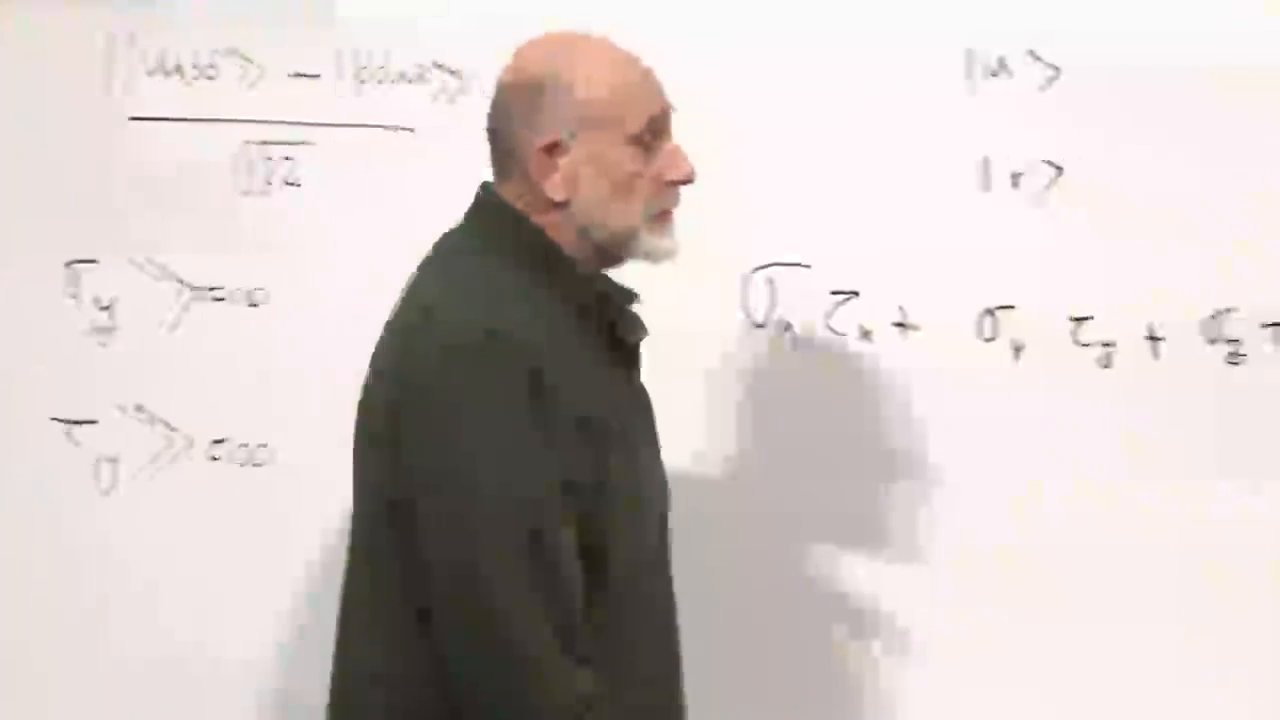
\includegraphics[width=0.88\textwidth]{lecture_07_figure_05.png}
\caption{回転不変な結合\(\boldsymbol{\sigma}\cdot\boldsymbol{\tau}\)と、一重項と三重項のセクターを分離する際のその役割。}
\lectureframe{00:52:33}
\end{figure}

相互作用ハミルトニアンが
\begin{equation}
H_{\mathrm{int}}
=J\,\boldsymbol{\sigma}\cdot\boldsymbol{\tau}.
\label{eq:l7-exchange-hamiltonian}
\end{equation}
を含むとしよう。反強磁性的結合\(J>0\)では、一重項は三重項より
\begin{equation}
\Delta E=4J.
\end{equation}
だけ低い。スピンを近づけ、より高いエネルギーの成分を光子、フォノン、その他の励起を放出して崩壊させると、対は一重項へと緩和する。その後、分離が制御されないスピン回転を導入したり、エネルギーギャップを急に閉じたりしない限り、結合状態を保ったままスピンを分離できる。

同じエネルギーの論理は原子系にも現れる。たとえばポジトロニウムでは、電子と陽電子のスピン結合が一重項配置と三重項配置を分裂させる。エネルギー差は\(E=mc^2\)を通じて質量差でもあるが、分光では通常、分裂をエネルギーまたは振動数として報告する。

\begin{classroomqa}
\audiencequestion{一重項は常に相互作用する二つのスピンの基底状態なのですか。}
\lecturerresponse{いいえ。それは式~\eqref{eq:l7-exchange-hamiltonian}における符号\(J>0\)に対する基底状態である。符号を逆にすると三重項の方が低くなる。生成の議論は、実際の相互作用とそのエネルギー順序に依存し、単に二つのスピンが存在することに依存するのではない。}
\end{classroomqa}

\begin{classroomqa}
\audiencequestion{\(\boldsymbol{\sigma}\cdot\boldsymbol{\tau}\)は三つの成分を別々に測定することで測定できますか。}
\lecturerresponse{一つの対に対して三つの同時局所スピン測定を行うことではできない。\(\sigma_x,\sigma_y,\sigma_z\)は非可換であり、三つの\(\tau\)成分も同様である。その期待値は\(x,y,z\)に沿って測定した三つの部分集団から再構成できるし、一重項--三重項観測量は適切な結合装置によって直接測定できる。}
\end{classroomqa}

\begin{classroomqa}
\audiencequestion{スピンが分離した後も、もつれを保つために相互作用し続けなければならないのですか。}
\lecturerresponse{いいえ。状態を生成または変化させるには相互作用が必要だが、いったん一重項が生成されれば、ユニタリ発展は粒子間に持続する力がなくてもそのもつれを保つことができる。局所磁場は二つの因子を回転させうるが、局所ユニタリ回転それ自体はもつれを破壊しない。}
\end{classroomqa}

\section{縮約密度行列}

アリスの局所期待値に戻ろう：
\begin{equation}
\expect{L_A}
=\sum_{a',a,b}
\Psi^*(a',b)L_{a'a}\Psi(a,b).
\end{equation}
\(L\)に属さない因子をまとめ直す：
\begin{equation}
\expect{L_A}
=\sum_{a',a}
\left[
\sum_b\Psi(a,b)\Psi^*(a',b)
\right]L_{a'a}.
\label{eq:l7-regrouped-expectation}
\end{equation}
括弧内の表式はアリスの縮約密度行列であり、
\begin{equation}
(\rho_A)_{aa'}
=\sum_b\Psi(a,b)\Psi^*(a',b).
\label{eq:l7-reduced-density-components}
\end{equation}
基底に依らない記法では、
\begin{equation}
\rho_A
=\operatorname{Tr}_B\ket{\Psi}\bra{\Psi},
\label{eq:l7-partial-trace}
\end{equation}
そしてすべてのアリス局所期待値は
\begin{equation}
\expect{L_A}
=\operatorname{Tr}_A(\rho_A L).
\label{eq:l7-density-expectation}
\end{equation}

\begin{figure}[htbp]
\centering
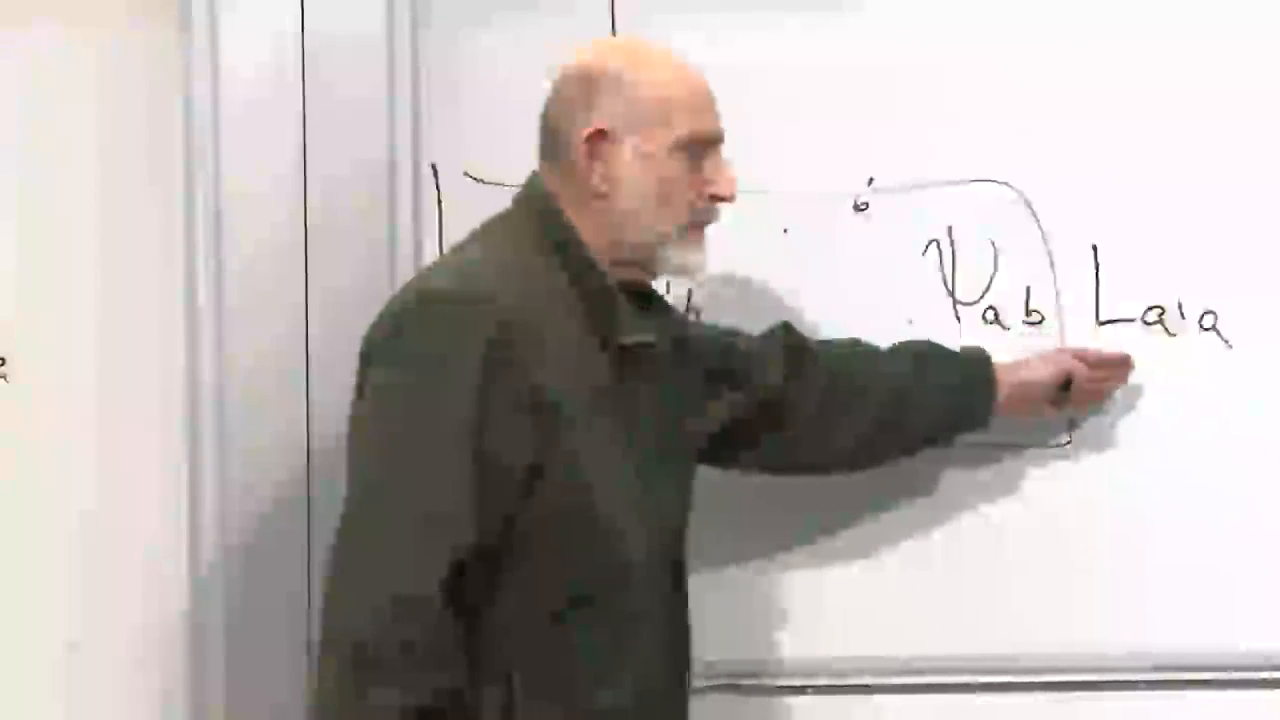
\includegraphics[width=0.88\textwidth]{lecture_07_figure_06.png}
\caption{ボブの基底ラベルについて結合振幅を総和して得られるアリスの密度行列。}
\lectureframe{01:02:33}
\end{figure}

縮約密度行列はエルミートで、正定値で、規格化されている：
\begin{equation}
\rho_A^\dagger=\rho_A,
\qquad
\bra{\chi}\rho_A\ket{\chi}\geq0,
\qquad
\operatorname{Tr}\rho_A=1.
\label{eq:l7-density-properties}
\end{equation}
これはアリスに限定されたすべての測定に必要な情報をちょうど含んでいる。二つの大域状態が同じ\(\rho_A\)を生じるなら、アリスのみの実験でそれらを区別することはできない。

\begin{classroomqa}
\audiencequestion{アリスは密度行列を一つの観測量として測定するのか？}
\lecturerresponse{一回の測定ではそうではない。密度行列は、すべての局所測定確率が計算されるもとになる対象である。同一に準備された多数の系が与えられれば、アリスはトモグラフィーによってそれを再構成できる。すなわち、十分な観測量の集合を測定し、それらの期待値から行列を推論する。}
\end{classroomqa}

\begin{classroomqa}
\audiencequestion{なぜボブの状態を一つ選ぶのではなく、ボブについて総和するのか？}
\lecturerresponse{アリスはボブから結果の情報を持たないからである。部分トレースは完全なボブ基底について総和し、無条件の局所状態を与える。代わりにボブの一つの結果を選ぶと条件付き状態が得られるが、これは異なる操作であり、その結果を知っていることを必要とする。}
\end{classroomqa}

積状態\(\Psi(a,b)=\psi_A(a)\phi_B(b)\)に対して、
\begin{align}
(\rho_A)_{aa'}
&=\sum_b
\psi_A(a)\phi_B(b)
\psi_A^*(a')\phi_B^*(b) \\
&=\psi_A(a)\psi_A^*(a')
\sum_b|\phi_B(b)|^2 \\
&=\psi_A(a)\psi_A^*(a').
\end{align}
したがって
\begin{equation}
\rho_A=\ket{\psi_A}\bra{\psi_A}.
\label{eq:l7-pure-projector}
\end{equation}
これは階数1の射影演算子である。\(\ket{\psi_A}\)に作用させると
\begin{equation}
\rho_A\ket{\psi_A}
=\ket{\psi_A}\braket{\psi_A}{\psi_A}
=\ket{\psi_A},
\label{eq:l7-density-on-state}
\end{equation}
一方、\(\ket{\psi_A}\)に直交するすべての\(\ket{\chi}\)に対して、
\begin{equation}
\rho_A\ket{\chi}
=\ket{\psi_A}\braket{\psi_A}{\chi}
=0.
\label{eq:l7-density-on-orthogonal}
\end{equation}

\begin{figure}[htbp]
\centering
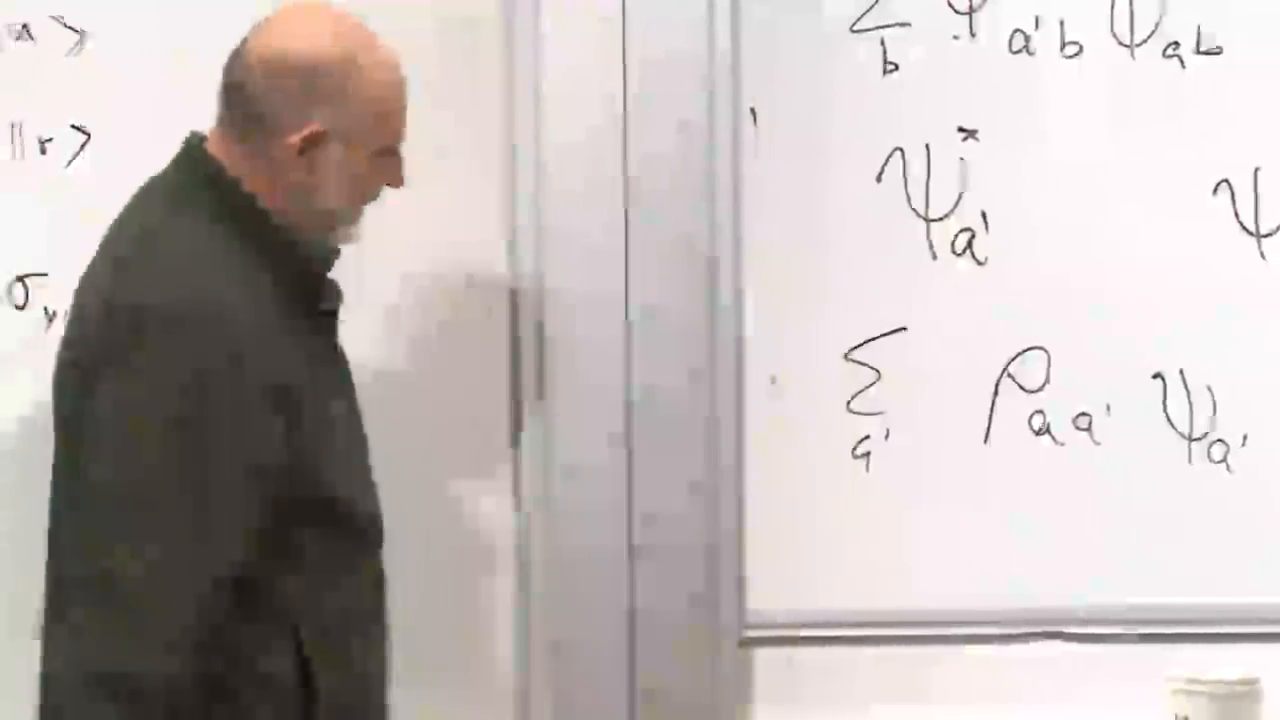
\includegraphics[width=0.88\textwidth]{lecture_07_figure_07.png}
\caption{射影演算子として作用する積状態の密度行列：\(\ket{\psi_A}\)に沿って固有値\(1\)、直交ベクトル上で\(0\)。}
\lectureframe{01:09:43}
\end{figure}

\section{密度行列のスペクトルとエンタングルメント}

\(\rho_A\)の固有値は非負であり、和は1である。全体の純粋状態に対して：
\begin{itemize}
\item 非零固有値がちょうど一つで、それが\(1\)に等しいなら、状態は積状態である；
\item 非零固有値が複数あるなら、状態はエンタングルしている；
\item 利用可能な局所サポート全体にわたって固有値が等しいなら、最大エンタングルメントを与える。
\end{itemize}
この主張はシュミット分解から最も明瞭である：
\begin{equation}
\begin{aligned}
\ket{\Psi}_{AB}
&=\sum_{r=1}^{R}\sqrt{\lambda_r}
\ket{r}_A\ket{r}_B,\\
\lambda_r&\geq0,
\qquad
\sum_r\lambda_r=1.
\end{aligned}
\label{eq:l7-schmidt}
\end{equation}
これに対して
\begin{equation}
\rho_A=\sum_{r=1}^{R}\lambda_r\ket{r}_A\bra{r}.
\label{eq:l7-schmidt-density}
\end{equation}
シュミット階数\(R\)は積状態では1であり、エンタングルした純粋状態では1を超える。

一重項に対して、
\begin{equation}
\rho_A
=\operatorname{Tr}_B\ket{S}\bra{S}
=\frac12\ket{u}\bra{u}
+\frac12\ket{d}\bra{d}
=\frac12 I.
\label{eq:l7-singlet-reduced-density}
\end{equation}
その固有値は
\begin{equation}
\operatorname{spec}(\rho_A)
=\left\{\frac12,\frac12\right\}.
\end{equation}
ペアの状態が純粋であっても、アリスの局所状態は最大混合である。

スペクトルは定量的な尺度を示唆する。フォン・ノイマンエントロピー
\begin{equation}
S(\rho_A)
=-\operatorname{Tr}(\rho_A\log\rho_A)
=-\sum_r\lambda_r\log\lambda_r
\label{eq:l7-entanglement-entropy}
\end{equation}
は積純粋状態で消え、\(d_A\leq d_B\)のとき最大エンタングル状態で\(\log d_A\)に達する。エントロピーの詳細な使用は後回しにしてよい。スペクトルはすでに本質的な区別を与えている。

\begin{classroomqa}
\audiencequestion{エンタングルした縮約密度行列の固有値はすべて非零でなければならないのか？}
\lecturerresponse{いいえ。非零固有値が複数あれば十分である。アリスの空間が大きい場合、エンタングルした状態はより低次元のシュミット部分空間のみを占め、追加の零固有値を残すことがある。最大エンタングルメントとは、より小さい部分系全体にわたって固有値が等しいことを意味し、任意に選んだ部分集合の間で等しいことではない。}
\end{classroomqa}

\begin{classroomqa}
\audiencequestion{混合した縮約密度行列それ自体が、アリスがボブとエンタングルしていることを証明するのか？}
\lecturerresponse{大域状態が純粋であると分かっている場合に限る。混合した局所状態は、混合した大域状態における通常の古典的混合からも生じうる。しかし純粋な二部分状態に対しては、局所的な混合性は二分割を横切るエンタングルメントと正確に等価である。}
\end{classroomqa}

\begin{classroomqa}
\audiencequestion{アリスの観測量のすべてのモーメントが彼女の確率分布を決定できるのか？}
\lecturerresponse{有限次元系では、演算子基底の期待値が\(\rho_A\)を決定し、\(\rho_A\)がボルンの規則を通じてすべての局所結果分布を決定する。再構成には同一に準備されたコピーの集団が必要であり、一つの孤立した事象が密度行列を明らかにすることはできない。}
\end{classroomqa}

\section{エンタングル相互作用としての測定}

アリスとボブをスピンと測定装置に置き換える。装置が準備状態\(\ket{0}_D\)とトリガー状態\(\ket{1}_D\)を持つとする。スピンが上向きかどうかを記録する理想的な相互作用は次で表せる：
\begin{align}
\ket{u}\ket{0}_D&\longrightarrow\ket{u}\ket{1}_D,\\
\ket{d}\ket{0}_D&\longrightarrow\ket{d}\ket{0}_D.
\label{eq:l7-measurement-basis-map}
\end{align}
検出器は既知の準備状態から始まらなければならない。そうでなければ、その最終状態は曖昧さのない記録を与えないであろう。

線形性が重ね合わせの時間発展を決定する：
\begin{equation}
\left(\alpha\ket{u}+\beta\ket{d}\right)\ket{0}_D
\longrightarrow
\alpha\ket{u}\ket{1}_D
+\beta\ket{d}\ket{0}_D.
\label{eq:l7-measurement-entanglement}
\end{equation}
一方の係数が消えない限り、最終状態はもつれている。装置が情報を得たのは、まさにその指針状態がスピンと相関しているからである。

\begin{figure}[htbp]
\centering
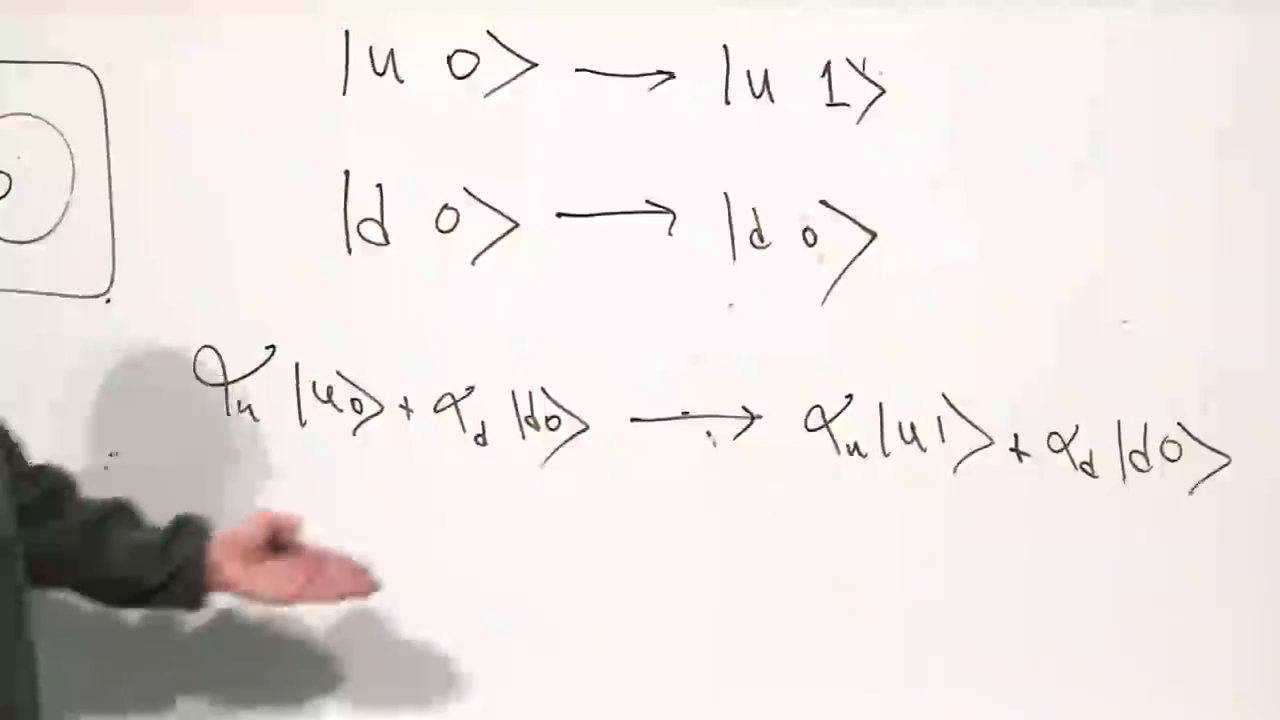
\includegraphics[width=0.88\textwidth]{lecture_07_figure_08.png}
\caption{理想測定はスピンの選択肢を異なる指針状態と相関させ、それによってもつれを生成する。}
\lectureframe{01:20:20}
\end{figure}

スピンだけを残し検出器を無視すると、その縮約状態は
\begin{equation}
\rho_{\mathrm{spin}}
=|\alpha|^2\ket{u}\bra{u}
+|\beta|^2\ket{d}\bra{d},
\label{eq:l7-postmeasurement-reduced-state}
\end{equation}
であり、指針記録が直交していると仮定している。干渉項は局所的な記述から消えている。それらは装置との相関の中に蓄えられているからである。

ここで二つの相補的な記述が存在する。検出器の結果を読み取り、記録に条件付けるなら、スピンには対応する枝が割り当てられる：トリガーの後なら\(\ket{u}\)、トリガーがなければ\(\ket{d}\)である。これが収縮の記述である。検出器とスピンを一つの閉じた系として扱うなら、式~\eqref{eq:l7-measurement-entanglement}は通常のユニタリー発展であり、結合状態からどの枝も取り除かれていない。

\begin{classroomqa}
\audiencequestion{測定はもつれを超えた何かだろうか？}
\lecturerresponse{系--装置のダイナミクスのレベルでは、測定とは信頼できる相関を確立する相互作用である。収縮は、確定した記録が選択された後に用いられる条件付きの記述である。その更新を根本的とみなすか、選ばれた切断に対して相対的とみなすかは解釈の問題であり、操作的予測は一致する。}
\end{classroomqa}

\begin{classroomqa}
\audiencequestion{なぜ理想測定はスピンの固有状態を変えないのか？}
\lecturerresponse{それがこの模型における再現性の要請である。入力がすでに測定される可観測量の固有状態なら、装置はその値を変えずに記録すべきである。現実の測定は破壊的でありうるが、その場合には相互作用を別様に模型化しなければならない。}
\end{classroomqa}

\section{観測者の階層}

装置を量子系として認めると、そこで止める自然な理由はない。指針からの光は目と相互作用し、目からの信号は脳と相関するようになり、観測者は別の観測者に観測されうる。Schr\"odingerの猫とウィグナーの友人は、同じ入れ子構造を劇的に示している：
\begin{equation}
\begin{gathered}
\text{spin}
\longrightarrow
\text{apparatus}
\longrightarrow
\text{cat}\\
\longrightarrow
\text{Schr\"odinger}
\longrightarrow
\text{Wigner}.
\end{gathered}
\label{eq:l7-observer-chain}
\end{equation}
選ばれた任意の境界の内側では、その連鎖をユニタリー発展と増大するもつれによって記述できる。境界の外側では、結果に条件付けられた収縮の言葉を用いる。

決定的な整合性条件は、境界を移動できることである。猫がスピン上を記録するなら、Schr\"odingerは後にスピン上を見た猫を記録しなければならず、ウィグナーはSchr\"odingerが同じ履歴を記録したことを記録しなければならない。量子力学は、客観的事象を宣言しなければならない唯一の鋭い線を特定しない。猫も目も脳も物理的自由度からできている。その一つを量子力学から除外するには、追加の法則が必要であろう。

そこから生じる不快感に対するファインマンの態度は実用的であった。概念的な問題はあまりに大きく、問題が存在するかどうかを述べることさえ難しいかもしれないが、計算規則はそれが適用されるあらゆる実験を予測し続ける。形式主義の目的は一つの解釈を強制することではなく、不快感の源を正確にすることである：全体についての完全な知識は、その部分についての純粋状態記述が存在しないことと共存しうる。

\begin{classroomqa}
\audiencequestion{もし私が猫なら、線を自分自身で引かなければならないのか？}
\lecturerresponse{自分に利用可能な確定した記録には収縮の記述を用いてよい。あなたをより大きな孤立系に含める別の観測者は、もつれた状態の記述を用いてよい。要求されるのは、全員が同じ線を引くことではなく、観測者が後に結果を比較するとき、すべての記述が整合した記録を与えることである。}
\end{classroomqa}

\begin{classroomqa}
\audiencequestion{客観的事象はどこで起こるのか：原子で、猫で、Schr\"odingerで、それともウィグナーで？}
\lecturerresponse{ユニタリー形式主義は、それらの場所の一つを特権的な境界として選び出さない。おそらく\emph{起こる}のような日常的な言葉は、それが正確である文脈を超えて押し広げられているのであろう。形式的な道具は、相関がどのように伝播し、各観測者が何を予測できるかを教えてくれる。最終的な境界をどう解釈するかを決めるのは別の課題である。}
\end{classroomqa}

\subsection{弱結合と不完全な読み出し}

式~\eqref{eq:l7-measurement-basis-map}の理想的な写像は完全に区別可能な記録を生み出す。より弱い相互作用では、装置の状態は部分的にしか区別できなくなるかもしれない：
\begin{equation}
\alpha\ket{u}\ket{D_u}
+\beta\ket{d}\ket{D_d},
\qquad
0<|\braket{D_d}{D_u}|<1.
\label{eq:l7-weak-measurement}
\end{equation}
そのとき装置は部分的な情報しか受け取らず、もつれは不完全である。これが弱測定または不鋭測定の設定である。

その状況は、下流の読み出しが不良であることとは区別されなければならない。検出器がスピンと完全に相関している一方で、目、ケーブル、増幅器、または脳が記録を正確に伝達できない場合がある。第一の場合、系--検出器相互作用は弱い。第二の場合、検出器には良好な記録が存在するが、その後の情報伝達が非効率的である。検出器効率はどちらの段階にも関わりうるので、原因を帰属させる前に物理的結合を特定しなければならない。

\begin{classroomqa}
\audiencequestion{視力が悪くて指針が不確かであるなら、その量子測定は弱測定だったのか。}
\lecturerresponse{必ずしもそうではない。スピンは装置と強く完全に相関していたかもしれないが、装置から目へ、あるいは目から脳への経路が不良であった。真に弱い測定とは、初期の系--装置結合そのものが部分的にしか区別できない記録しか生み出さなかったことを意味する。}
\end{classroomqa}

\section{局所性とノーシグナリング}

\emph{遠隔作用}という語には操作的な意味を与えるべきである。通常の物理学では、遠方の作用はここで観測できるものを変える。もし太陽が消え、光の伝播時間の後ではなく直ちに地球の運動が変化したなら、その変化を利用して光より速く情報を伝達できるであろう。それが真の非局所的なシグナリングである。

エンタングルメントはそのようなシグナリングを許さない。ボブがクラウス演算子\(K_\mu\)で表される局所量子操作を行い、
\begin{equation}
\sum_\mu K_\mu^\dagger K_\mu=I_B.
\end{equation}
とする。アリスがボブの結果を知らない場合、最終的な結合状態は
\begin{equation}
\rho'_{AB}
=\sum_\mu
(I_A\otimes K_\mu)\rho_{AB}
(I_A\otimes K_\mu^\dagger).
\end{equation}
であり、ボブについて部分トレースを取ると
\begin{equation}
\rho'_A
=\operatorname{Tr}_B\rho'_{AB}
=\operatorname{Tr}_B\rho_{AB}
=\rho_A.
\label{eq:l7-no-signaling}
\end{equation}
となる。したがって、無条件のアリス局所確率は、ボブのトレース保存局所操作の選択によって変わらない。

条件付き状態は異なる。ボブが測定して結果\(\mu\)を得たなら、アリスは
\begin{equation}
\rho_{A|\mu}
=\frac{
\operatorname{Tr}_B\!\left[
(I_A\otimes K_\mu)\rho_{AB}
(I_A\otimes K_\mu^\dagger)
\right]
}{p_\mu}.
\label{eq:l7-conditioned-state}
\end{equation}
を割り当てることができる。しかしアリスは、ボブが通常の信号によって\(\mu\)を伝えるまで、どの\(\rho_{A|\mu}\)が当てはまるかを知ることができない。メッセージが届く前には、彼女は結果について平均しなければならない：
\begin{equation}
\sum_\mu p_\mu\rho_{A|\mu}=\rho_A.
\label{eq:l7-conditioned-average}
\end{equation}

\begin{classroomqa}
\audiencequestion{ボブが先に測定した場合、アリスの密度行列はいつ変化するのか。}
\lecturerresponse{彼女の無条件密度行列は変化しない。ボブの結果が彼女に届いた後、彼女はそれを対応する条件付き密度行列で置き換えてよい。その更新は新たに利用可能になった情報を反映しており、古典的メッセージが届く前に用いることはできない。}
\end{classroomqa}

\begin{classroomqa}
\audiencequestion{ボブの測定は、同じ瞬間にアリスの状態を物理的に収縮させるのか。}
\lecturerresponse{異なる解釈は条件付き更新を異なる仕方で記述するが、検証可能な命題についてはすべて一致する。すなわち、ボブからの情報が利用可能になるまで、アリスの局所的な結果確率は変わらない。制御可能な瞬間的シグナルは生じない。}
\end{classroomqa}

多数の一重項対が番号付きの行に分配されていると想像しよう。一方の構成要素ではボブは\(z\)を測定し、別のものでは\(x\)を、また別のものでは\(y\)を測定する、という具合である。アリスの局所的な結果はどの行についても偏りのない系列のままである：
\begin{equation}
P_A(+|\mathbf a)=P_A(-|\mathbf a)=\frac12.
\label{eq:l7-alice-marginal}
\end{equation}
彼女のノートには、ボブがどの軸を選んだか、どの結果を得たかを明かすものは何もない。

\begin{figure}[htbp]
\centering
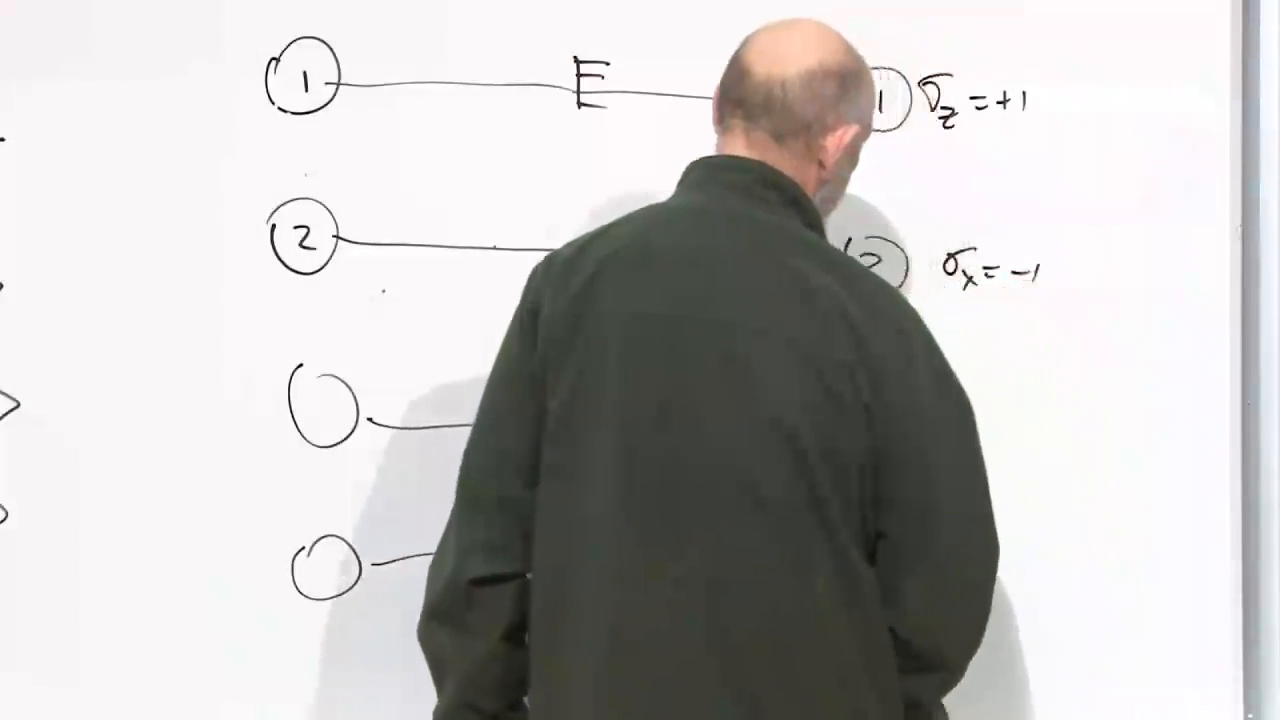
\includegraphics[width=0.88\textwidth]{lecture_07_figure_09.png}
\caption{多数の独立に準備された対があれば、異なる測定軸を異なる行に割り当てることができるが、アリスの周辺統計は変わらない。}
\lectureframe{01:49:00}
\end{figure}

光速で制限された電報が届き、各行についてボブの軸と結果が列挙された後、アリスは自分の記録を並べ替えることができる。同じ軸での一重項測定は、そのとき対ごとに反対になる。そのメッセージは結合統計にすでに存在する相関を明らかにするのであって、アリスの以前の局所的な頻度分布を遡って変えるのではない。

\begin{classroomqa}
\audiencequestion{アリスは、自分のデータの十分に多くのモーメントからボブの選択を推論できるか。}
\lecturerresponse{できない。アリス局所的なすべてのモーメントは\(\rho_A\)によって固定されており、式~\eqref{eq:l7-no-signaling}はその行列を変えない。より多くのコピーは同じ局所密度行列の推定を改善するだけで、ボブの基底や結果を明かすものではない。}
\end{classroomqa}

\begin{classroomqa}
\audiencequestion{ボブがアンサンブルの各構成要素で異なる軸を選ぶ場合はどうか。}
\lecturerresponse{アリスは依然として同じ局所分布を見る。ボブが行ごとの設定と結果を送った後、両者は各軸の対について条件付き相関を比較できる。設定依存性は結合統計に現れ、アリスの周辺統計には現れない。}
\end{classroomqa}

\section{シミュレーションゲームとしてのベルの問い}

シグナリングが存在しないこととベル非局所性の区別は、古典的シミュレーションの問題としてより明確になる。まず1つのスピンから始める。
\begin{equation}
\ket{\psi}=\alpha_u\ket{u}+\alpha_d\ket{d},
\qquad
|\alpha_u|^2+|\alpha_d|^2=1.
\end{equation}
古典的なプログラムは2つの複素振幅を保存し、それらをSchr\"odinger方程式で時間発展させ、ユーザーが選択した測定方向を受け入れることができる。測定コマンドが発行されると、プログラムはボルンの確率を計算し、擬似乱数生成器を用いて結果を選び、その結果を表示し、保存された状態を対応する固有状態に更新する。この過程を繰り返すことで、1つのスピンの統計が再現される。

したがって、ランダム性だけが古典力学と量子力学を分ける境界線ではない。古典的なコンピュータは、その擬似乱数アルゴリズムが根底では決定論的であっても、シミュレーションに十分なほど操作的にランダムな列を生成できる。

積状態にある2つのスピンに対しては、離れた2台のコンピュータでも十分である。アリスのコンピュータは\(\ket{\psi_A}\)を保存して時間発展させ、ボブのコンピュータは\(\ket{\phi_B}\)を保存して時間発展させる。それぞれは自分の局所的な設定にのみ応答する。結合確率が因数分解するため、コンピュータが分離された後には通信は必要ない。

もつれた対は問題を変える。実験の前に2台の機械を一緒にし、相関した隠れたデータを読み込み、それらの時計を同期させ、さらに同一の乱数シードを与えることさえできる。しかし、分離後には、各出力は自分の局所的な測定設定と事前に与えられた共有情報にのみ依存しなければならない。ベルの定理は、そのような局所隠れ変数スキームでは、自由に選ばれた設定に対するすべての量子相関を再現できないことを示している。

\begin{figure}[htbp]
\centering
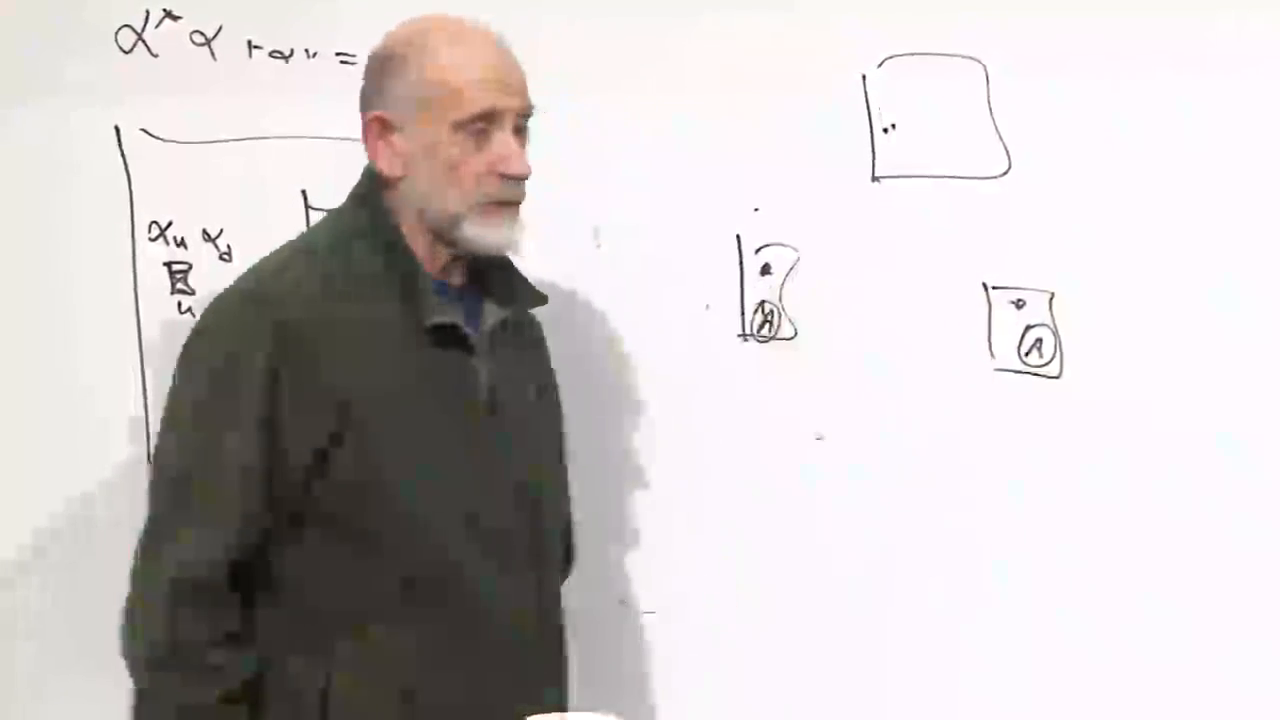
\includegraphics[width=0.88\textwidth]{lecture_07_figure_10.png}
\caption{分離したコンピュータのモデル：局所的なプログラムは準備データを共有してよいが、分離後には測定設定を通信できない。}
\lectureframe{02:00:00}
\end{figure}

設定と結果を交換できるようにコンピュータ間に配線が残っているならば、シミュレーションは相関を再現できる。しかしその場合、その対はもはや真に分離した局所モデルではなく、1台の接続されたコンピュータとして機能する。障害は抽象的な古典計算にあるのではない。単一の大域的な古典的機械は、完全な結合波動関数を保存することにより有限の量子系をシミュレートできるが、必要なメモリは一般に部分系の数とともに指数関数的に増大する。ベルの障害は、独立に動作する局所的な機械への分解に関するものである。

\begin{classroomqa}
\audiencequestion{なぜ2台のコンピュータは単に同じ乱数列を使えないのか。}
\lecturerresponse{共有乱数はすでに局所隠れ変数モデルで許されている。それは相関した答えを事前に決定できるが、各答えは、その側で後から選ばれる可能性のあるあらゆる測定設定に対して機能しなければならない。ベル不等式は、そのようなすべての事前に取り決められた局所戦略が従う制約を表しており、量子相関はそれらの制約に違反する。}
\end{classroomqa}

\begin{classroomqa}
\audiencequestion{乱数は測定方向に依存しなければならないのか。}
\lecturerresponse{局所的な出力は、自分の局所的な方向と共有された隠れたデータに依存してよいが、分離後に選ばれた遠方の方向には依存しない。両方の設定への依存を許すには、通信、逆行因果性、または通常の測定独立性の仮定の破れが必要である。ベルの定理は、これらの仮定を\emph{ランダム}という語の中に隠すのではなく、明示する。}
\end{classroomqa}

\begin{classroomqa}
\audiencequestion{古典的なプログラムが失敗するのに対し、離れた2台の量子コンピュータは成功するのか。}
\lecturerresponse{それらがもつれた量子的自由度を共有していれば成功しうる。その場合、コンピュータは局所的な古典的記録でもつれをシミュレートしているのではなく、もつれを物理的に持っている。それらの局所的な結果は依然として、制御可能な超光速メッセージを伝送することはできない。}
\end{classroomqa}

\begin{classroomqa}
\audiencequestion{1台の通常の古典的コンピュータで対全体をシミュレートできるか。}
\lecturerresponse{できる。それは4つの結合振幅を保存し、すべての測定確率を1か所で計算できる。多数の粒子に対しては、ヒルベルト空間の次元が指数関数的に増大するため、この直接シミュレーションは高コストになるが、すべての情報が1台の機械の内部で大域的に利用可能である場合、ベルの矛盾は存在しない。}
\end{classroomqa}

\begin{classroomqa}
\audiencequestion{それでは、ベルの定理は通常の遠隔作用を証明するのか。}
\lecturerresponse{それは、ベルの仮定を満たす局所隠れ変数による説明が観測された相関を再現できないことを証明する。それはアリスやボブに超光速シグナリング経路を与えるものではない。ベル非局所性と操作的な超光速通信は別個の主張である。}
\end{classroomqa}

\section{局所的に何を学べるか}

局所的な観測量と結合観測量を混同してはならない。ボブは\(\sigma_x\)を測定でき、アリスは\(\tau_x\)を測定できる。後に記録を比較することで、彼らは
\begin{equation}
\expect{\sigma_x\tau_x}.
\end{equation}
を推定する。どちらの局所装置も単独ではその積を測定しない。回転スカラー
\begin{equation}
\boldsymbol{\sigma}\cdot\boldsymbol{\tau}
=\sigma_x\tau_x+\sigma_y\tau_y+\sigma_z\tau_z
\end{equation}
には、三つの項に対して異なる部分集団を用いるか、一重項と三重項のセクターを分解する新しい結合装置が必要である。元の局所スピン計を用いて一対から三つの非両立な成分の積すべてを得ることはできない。

\begin{classroomqa}
\audiencequestion{アリスとボブの元の装置が別々には測定できない全体の観測量は存在するか。}
\lecturerresponse{はい。\(\sigma_x\tau_x\)のような単一の積は、二つの局所\(x\)測定の後に比較することで推定できる。和\(\boldsymbol{\sigma}\cdot\boldsymbol{\tau}\)は、一対に対する同時\(x,y,z\)読み取りから組み立てることはできない。それには真に結合した一重項--三重項測定か、非両立な項のための別々の集団が必要である。}
\end{classroomqa}

ボブは一回の事象からもつれを推論することはできない。しかし、同一に準備された多数のコピーがあれば、彼は自分の縮約密度行列を再構成できる。量子ビットに対して、
\begin{equation}
\rho_B
=\frac12\left(
I+\mathbf r\cdot\boldsymbol{\sigma}
\right),
\label{eq:l7-bloch-density}
\end{equation}
であり、いくつかの軸に沿った測定がブロッホベクトル\(\mathbf r\)を決定する。\(|\mathbf r|=1\)ならば、ボブの局所状態は純粋であり、\(|\mathbf r|<1\)ならば混合である。大域的な準備が毎回同じ純粋状態であることが知られている特別な場合には、局所的な混合性は、ボブが自分の部分系の外の何かともつれていることを証明する。

二つの純粋スピンの積に対して、ボブは偏極方向\(\mathbf n=\mathbf r/|\mathbf r|\)を探すことができる。その軸に沿って、繰り返し測定は一つの確定した答えを返す。一重項では\(\mathbf r=0\)であるため、どの軸も局所的にランダムなままである。探索は偏極方向を決して見つけない。

\begin{classroomqa}
\audiencequestion{ボブはアリスと話さずにもつれを発見できるか。}
\lecturerresponse{集団から、彼は自分の縮約状態が混合であることを発見できる。また、すべての対が同じ大域的純粋状態に準備されたことを知っていれば、彼は境界を越えたもつれを推論できる。その純粋性の仮定がなければ、彼の混合状態は代わりに古典的な準備の混合から生じる可能性があり、局所データだけではその区別を決着できない。}
\end{classroomqa}

\begin{classroomqa}
\audiencequestion{なぜ同一に準備された多数の系が必要なのか。}
\lecturerresponse{各スピン測定は一つの結果しか与えず、一般にそのコピーを乱す。したがってトモグラフィーは、非両立な測定を同じ手順で準備された集団全体に分配する。密度行列とそのスペクトルは、それらの繰り返し試行から推論される統計的性質であり、一つの粒子によって明かされるラベルではない。}
\end{classroomqa}

論理は今、それが始まったところで閉じる。もつれとは、状態の漠然とした共有ではない。それは、純粋な結合状態が因数分解できないことであり、局所的には射影子でない縮約密度行列として、結合的には分離した古典的記帳では再現できない相関として現れる。全体が完全に知られていても、各部分は混合のままでありうる。その事実が測定を可能にし、シグナル伝達が起こらないことを保ち、ベル定理が検証することになる構造を与える。
